\section{Verifying Isosurface Extraction Algorithms}
\label{chap1:sec:iea}

In this section, we describe the technique we use for verifying
isosurface extraction algorithms, namely the \emph{method of manufactured
solutions} (MMS). We illustrate a possible implementation of MMS in
Algorithm~\ref{alg:manufactured-solutions} and Figure ~\ref{fig:mms-flow}. This 
technique requires us to write down the expected behavior of particular 
features of interest of the object (or model problem) 
being generated. In our case, we are generating triangular
approximations of smooth isosurfaces, and the features of interest are
geometric surface convergence, convergence of normals, area and
curvature. 

\begin{algorithm}[h]
\begin{codebox}
\Procname{$\proc{MMS}(f, u, h_1)$}
\li \Comment Let $f$ be a scalar field containing the solution surface $S$
\li \Comment Let $u$ be a given property ($f$, normals, area, etc.)
\li \Comment Let $h_1$ be the initial grid size
\li \For $i \gets 1$ \To $n$
\li     \Do $G_{h_i} \gets $ an approximation of $f$ at grid size $h_i$
\li         $S_{h_i} \gets $ an approximation of $S$ computed from $G_{h_i}$
\li         $E_{h_i} \gets || u(S_{h_i}) - u(S)||_u$
\li         $x_i \gets \log h_i$, $y_i \gets \log E_{h_i}$
\li         $h_{i+1} \gets h_i / 2$
        \End
\li $\tilde{q} \gets $ slope of best-fit linear regression of $(x_i, y_i)$
\li Compare $\tilde{q}$ and $q$
\end{codebox}
\caption{\label{alg:manufactured-solutions}Overview of the method of manufactured solutions (MMS).}
\end{algorithm}

To use MMS, we first accomplish a mathematical analysis of
the expected convergence rate of the features (or characteristics) of interest, 
known in the numerical literature as the \emph{formal order of accuracy} of the
characteristic. This analysis is done for solutions of the problem that can
be conveniently described and analyzed (these are the manufactured
solutions). Then, the code is executed with progressively refined
versions of the data that is used in the generation or sampling of 
the manufactured solution. Finally, the empirical convergence rate is compared to the
one predicted by the analysis.  When the convergence rates are
comparable, we increase our confidence in the algorithm.
%
If the realizable behavior disagrees with the analysis, either (1) the analysis 
does not correspond to the correct behavior of the algorithm, (2) the assumptions
upon which the analysis was build were violated by the input data and hence
the predicted behavior is not valid for the circumstances under investigation, or (3) 
there are issues with the algorithm or with the implementation of the 
algorithm (depending on access to source code
and algorithmic details, one may not be able to distinguish between
these two -- algorithmic or implementation -- and hence we in this work 
always consider them together. Given sufficient information, the
verification process can help further delineate between these
two issues). Notice, however, that all three situations
warrant further investigation. In the following sections, we will discuss
these issues in more detail.  Let us first clarify how
we will arrive at theoretical and empirical convergence rates.

For a fixed grid size, we will strive to write the approximation error
between the desired isosurface property and its approximation by:
\begin{equation}
E = |u_{approx} - u_{exact}|_u = O(h^p) = \alpha h^p
\label{eq:theoretical-convergence-rate}
\end{equation}
\noindent where $u_{approx},u_{exact}$ are the approximated and 
exact values of a property $u$,  
$|\cdot|_u$ is the norm used to compare the approximate and exact property,
$p$ is the order of accuracy and $\alpha$ is a constant. 
Practically speaking, the polynomial expression
(\ref{eq:theoretical-convergence-rate}) is not very convenient for numerical 
experimentation, as 
it is hard to find the value of $p$ from the direct plot of $h$ against $E$.
The standard technique to estimate $p$ is to linearize by
working on a log-log scale:
\begin{equation}
 \log E = \log (\alpha  h^p) = \log \alpha  + p \log h.
\label{eq:error-log-evaluation}
\end{equation}

Using this linearized version, we estimate $p$ from the slope of 
the line that best fits the points $(\log h,\log E)$ in a
least-squares sense. We use this technique in Section~\ref{chap1:sec:res}
when testing the isosurface codes.

\begin{figure}[t]
\centering
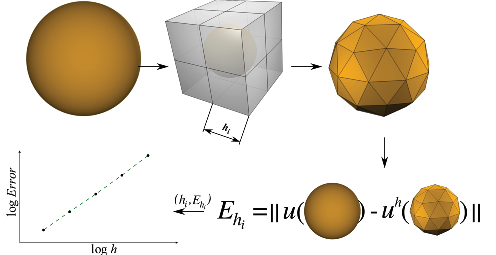
\includegraphics[width=0.95\linewidth,keepaspectratio=true]{chapter2/figures/mms.pdf}
\caption{\label{fig:mms-flow}Workflow for the method of manufactured solution (Algorithm \ref{alg:manufactured-solutions}), clockwise from the top left.}
\end{figure}

MMS critically depends on an analysis of the order of accuracy of
expected solutions. Although this seems quite simple, the order of
accuracy under a sensitive norm like $||\cdot||_\infty$ has shown in
practice to be very effective in bringing out implementation errors in
numerical approximation schemes~\cite{Roy2005,babuska04}. In this
dissertation, we show that this analysis is just as effective for isosurface
extraction. In addition, we believe the convergence analysis required
by MMS is interesting in its own right. As we will discuss in
Section~\ref{chap1:sec:dis}, it helps to shed light on the consequences of
implementation choices.

In the context of isosurface methods, manufactured solutions can be built by
specifying a ``solution surface'' to be the exact solution and deriving a 
scalar field that contains such a solution surface as a level set. The 
verification methodology then proceeds as following: 
(1) use the manufactured scalar field as input for the isosurfacing 
methods, (2) run the methods, and (3) check the output surface against 
the solution surface (sometimes called the {\em ansatz solution} within
the mathematical verification literature).
In many cases, the manufactured scalar field can be derived analytically, 
making the observed order of accuracy tractable (we give
examples in next section).

%% The overall methodology for
%% verifying isosurface tools through manufactured solution can be stated as follows:
%algorithm \ref{alg:manufactured-solutions} presents the overall methodology for verifying
%isosurface tools using the method of manufactured solution. Details
%about how to computed the errors involved in the convergence analysis
%will also be given in next section.
%% In Algorithm~\ref{alg:manufactured-solutions} given above, $\tilde{q}$ and $q$ are the observed and 
%% analytical order of accuracy. Details about the metric $|\cdot|_u$ will be given in next section. 

%% \subsection{Formal order of accuracy}

%% Order of accuracy aims at deriving a mathematical framework
%% towards understanding, from a theoretical point of view, 
%% at which rate the approximations errors generated by isosurfacing schemes converge to the real isosurface 
%% when successive refinement is applied in the background domain.
%% More specifically, we analyze how the approximate vertices, normals, area, and curvatures
%% tend to their exact counterparts when ``finer and finer'' background grids are employed. 

In what follows, we will derive expected orders of accuracy for
several features of surfaces produced by isosurface extraction codes. We keep
our assumptions about the actual algorithms to a minimum to maximize
the applicability of the arguments given. We essentially only assume
that the maximum triangle size can be bounded above at any time, and
use Taylor series arguments (under assumptions of smoothness) 
to derive convergence rates. 
%
It is important to point out that order of accuracy analysis of
polyhedral surfaces has been studied by many
researchers~\cite{meek2000,xu2006,zxuLNCS05,hildebrandt06}.  In
fact, the results presented below are in agreement with the ones
reported in the literature. However, because we are considering
isosurface extraction, some of our arguments benefit by being
able to be condensed to simpler statements.

\subsection{Convergence of Vertex Position}
\label{subchap1:sec:vertex-order-of-accuracy}

We start our analysis of isosurface extraction by studying the
convergence of vertex positions. We analyze this convergence
indirectly by relating the values of the scalar field at the vertex
points and the distance between the vertices and the correct
isosurface. Given a value $\lambda$ such that the exact isosurface $S$
is defined by $f(x,y,z) = f(\vec{v}) = \lambda$, the \emph{algebraic}
distance of $\vec{v}$ to $S$ is defined as $|f(\vec{v}) - \lambda|$
\cite{Taubin94}. Notice that algebraic distances only makes sense
for implicit surfaces: it requires a scalar field. In addition, 
we restrict ourselves to \emph{regular} isosurfaces,
ones where for every point $x$ in $S$, $|\nabla f(x)|$ exists and
is nonzero.
%
Then, the geometric distance between
$\vec{v}$ and $S$ is approximated by $|f(\vec{v}) - \lambda| / |\nabla
f(\vec{v})|$ \cite{Taubin94}. We illustrate this relation
in Figure \ref{fig:algebraic-distance}. Since, by assumption, 
$|\nabla f(x)| > k$ for some
$k > 0$, and all $x$ in $S$, convergence in algebraic distance implies convergence in
geometric distance. Convergence in algebraic distance, however, is much
more tractable mathematically, and this is the item to which we turn our focus.

Many isosurface methods estimate vertex positions through linear
interpolation along edges of a grid.
Let $f:U\subset\mathbb{R}^3 \rightarrow \mathbb{R}$ be the a smooth 
real function defined in a 
subset $U=[a_x,b_x]\times[a_y,b_y]\times[a_z,b_z]$, where $[a_i,b_i], i \in {x,y,z}$ 
are real intervals.
We assume the intervals $[a_i,b_i]$ have the same length and 
let $a_x=x_0,\ldots,x_n=b_x$, $a_y=y_0,\ldots,y_n=b_y$, and
$a_z=z_0,\ldots,z_n=b_z$ be subdivisions for the intervals such that
$x_i = x_0+ih$, $y_i = y_0+ih$, $z_i = z_0+ih,\, i=0,\ldots,n$, 
where $h$ is the grid size and 
$c_{ijk}=[x_i,x_{i+1}]\times[y_j,y_{j+1}]\times[z_k,z_{k+1}]$
is a grid cell. 
\begin{figure}[h]
\centering
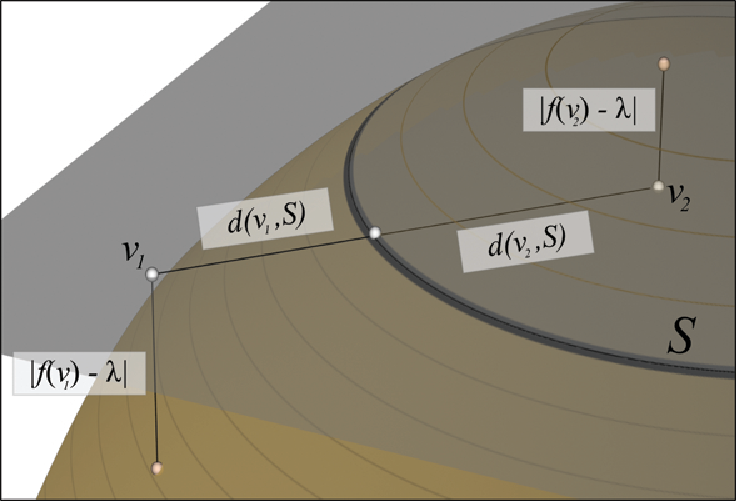
\includegraphics[width=.5\linewidth]{chapter2/figures/algebraic.pdf}
\caption{The distance between a point $\vec{v}$ and the isosurface $S$
  with isovalue $\lambda$ can be approximated by the algebraic
  distance divided by the gradient magnitude of the scalar field at $\vec{v}$,
  $|f(\vec{v})-\lambda| / |\nabla f(\vec{v})|$. In the figure, the
  thick circle represents the isosurface $S$ and the fainter isolines
  illustrate changes in gradient magnitude: in regions of small
  gradient magnitude, the algebraic distance is small but geometric
  distance is large, and vice-versa for large gradient magnitude.}
\label{fig:algebraic-distance}
\end{figure}
Through a Taylor series expansion of $f$, one can evaluate $f$ 
at a point $\vec{p}\in c_{ijk}$ as:
\begin{equation}
f(\vec{p}) = f_{ijk} + \nabla f_{ijk}\cdot \vec{\delta} + \frac{1}{2}\vec{\delta}^T H(\vec{\xi}) \vec{\delta}
\label{eq:taylor}
\end{equation}
\noindent where $f_{ijk}=f(x_i,y_j,z_k)$, $\nabla f_{ijk}$ is the gradient 
of $f$ in $(x_i,y_j,z_k)$,
$H(\vec{\xi})$ is the Hessian of $f$ at a point $\vec{\xi}$ 
connecting $(x_i,y_j,z_k)$ and $\vec{p}$, 
and $\vec{\delta} = (u,v,w)^T$ is such that $\vec{p} = (x_i+uh,y_j+vh,z_k+wh)^T$.

Let the linear approximation of $f$ in $\vec{p}$ be defined by
\begin{equation}
\tilde{f}(\vec{p}) = f_{ijk} + \nabla f_{ijk}\cdot \vec{\delta}
\label{eq:linear}
\end{equation}
\noindent and consider a point $\vec{x_\lambda}$  such that $\tilde{f}(\vec{x_\lambda}) = \lambda$, that is,  
$\vec{x_\lambda}$ is a point on the isosurface $\lambda$ of $\tilde{f}$.

The algebraic distance between the exact isosurface $f(x,y,z) = \lambda$ and
the linearly approximated isosurface can be measured by 
$|f(\vec{x_\lambda}) - \lambda|$. From Equations~\ref{eq:taylor} and~\ref{eq:linear} one can 
see that
\begin{equation}
\begin{array}{c}
\displaystyle{|f(\vec{x_\lambda}) - \lambda| = |f_{ijk} + \nabla f_{ijk}\cdot \vec{\delta} + \frac{1}{2}\vec{\delta}^T H(\vec{\xi}) \vec{\delta} -\lambda| =}\\
|\tilde{f}(\vec{x_\lambda}) + O(h^2) -\lambda| = O(h^2)
\end{array}
\label{eq:algebraicerror}
\end{equation}
\noindent thus, the linearly approximated isosurface is of second-order accuracy.

%% Algebraic error has been adopted as one of the verification mechanisms presented in next section. We have opted
%% by algebraic error rather than geometrical error because the former is as much effective as geometrical 
%% error in the context of verification while still being computationally less expensive to compute.

%\noindent the approximation error can be written as:
%\begin{equation}
%|f(\vec{p}) - \tilde{f}(\vec{p})| = |\frac{1}{2}\vec{\delta}^T H(\vec{\xi}) \vec{\delta}| = O(h^2).
%\label{eq:linearerror}
%\end{equation}

%As isosurfacing methods place the vertices of the approximate isosurface on a level set of $\tilde{f}$, 
%these approximate vertices
%should converge to the real isosurface at the same rate as $\tilde{f}$ converges to $f$.
%In the case of linear interpolation, the rate of 
%convergence is quadratic, as one can be seen from Equation (\ref{eq:linearerror}).

\subsection{Convergence of Normals}
\label{chap1:sec:normalconvergence}

Assume, generally, that the scalar field $f(x,y,z)=\lambda$ can be
locally written as a graph of a function in two-variables
$g(x(u,v),y(u,v))=\lambda-f(x(u,v),y(u,v),z_k)$, as illustrated in
Figure~\ref{fig:graphfunct}, where $x(u,v) = x_i+uh$ and
$y(u,v)=y_j+vh$. This is acceptable because we have already assumed
the isosurface to be regular. Still without losing generality we
write $g(x(0,0),y(0,0)) = 0$, that is, the isosurface
contains the point $(x_i,y_j,z_k)$.
\begin{figure}[b]
  \centering
  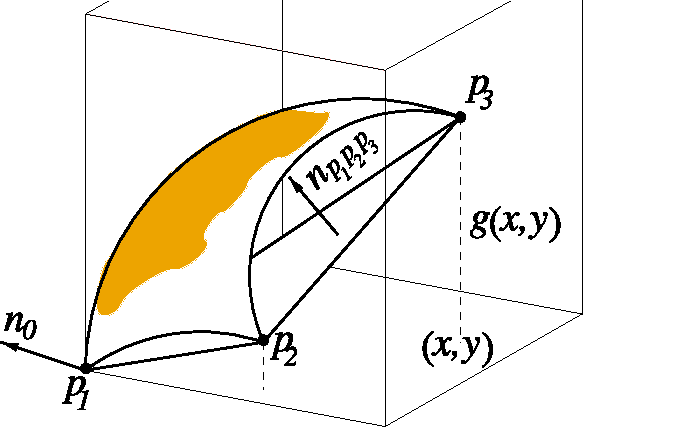
\includegraphics[width=0.40\linewidth,keepaspectratio=true]{chapter2/figures/gridcell.pdf}
  \caption{Isosurface local parametrization and approximation.}
  \label{fig:graphfunct}
\end{figure}
 Let  $\vec{\Phi}(u,v) = (x(u,v),y(u,v),g(x(u,v),y(u,v)))$ be a parametrization 
for the isosurface $f(x,y,z)=\lambda$ in $c_{ijk}$ and
% \begin{equation}
% \frac{\partial\vec{\Phi}}{\partial u}\times\frac{\partial\vec{\Phi}}{\partial v} = 
% h^2\left(\begin{array}{c}
%              -\frac{\partial g}{\partial x}\\
% 	     -\frac{\partial g}{\partial y}\\ 
% 	     1\end{array}\right) = h^2 \vec{n_0}
% \label{eq:normal_exact}
% \myspacemini
% \end{equation}
\begin{equation}
\frac{\partial\vec{\Phi}}{\partial u}\times\frac{\partial\vec{\Phi}}{\partial v} = 
h^2\left(-\frac{\partial g}{\partial x},\\
	     -\frac{\partial g}{\partial y},\\ 
	     1\right)^T = h^2 \vec{n_0}
\label{eq:normal_exact}
\end{equation}
\noindent be the normal vector in $\vec{\Phi}(0,0)=(x_i,y_j,g(x_i,y_j))$ 
(the partial derivatives of $g$ are evaluated at $(x(0,0),y(0,0))=(x_i,y_j)$).

Consider now the triangle defined by the points $\vec{p_1},\vec{p_2}$, and $\vec{p_3}$ 
approximating the isosurface
$f(x,y,z)=\lambda$ in the grid cell $c_{ijk}$ (see Figure~\ref{fig:graphfunct}).
Let $\vec{p_1}$ be the grid point $(x_i,y_j,z_k)$, so $\vec{p_1}=\vec{\Phi}(0,0),\, \vec{p_2}=\vec{\Phi}(u_2,v_2)$, and $\vec{p_3} = \vec{\Phi}(u_3,v_3)$. 
Using the cross product in $\mathbb{R}^3$, 
the normal of the triangle $p_1p_2p_3$ can be computed by:
\begin{equation}
\begin{array}{c}
\displaystyle{\vec{n_{p_1p_2p_3}}\!\! =\!\! (\vec{p_2} - \vec{p_1})\times(\vec{p_3} - \vec{p_1})\!\! =} \\
\displaystyle{\left(\!\!\!\!\!\begin{array}{c}
h(v_2g(x(u_3,v_3),y(u_3,v_3)) - v_3g(x(u_2,v_2),y(u_2,v_2)))\\
h(u_3g(x(u_2,v_2),y(u_2,v_2)) - u_2g(x(u_3,v_3),y(u_3,v_3)))\\
%h(u_3g(u_2,v_2) - u_2g(u_3,v_3))\\
h^2(u_2v_3-u_3v_2))
\end{array}\!\!\!\!\!\right).}
\end{array}
\label{eq:normal_tri1}
\end{equation}

Expanding $g(x(u_i,v_i),y(u_i,v_i)),\, i \in \{2,3\}$ in a Taylor
series, some terms cancel and the normal $\vec{n_{p_1p_2p_3}}$ becomes:
% \begin{equation}
% \vec{n_{p_1p_2p_3}} = rh^2
% \left(\begin{array}{c}
% -\frac{\partial g}{\partial x} + O(h)\\
% -\frac{\partial g}{\partial y} + O(h)\\ 
%  1\end{array}\right)
% \label{eq:normal_tri2}
% \myspacemini
% \end{equation}
\begin{equation}
\vec{n_{p_1p_2p_3}} = rh^2
\left(
-\frac{\partial g}{\partial x} + O(h),\\
-\frac{\partial g}{\partial y} + O(h),\\ 
 1\right)^T
\label{eq:normal_tri2}
\end{equation}
where $r = u_2v_3-u_3v_2$. 
Comparing the exact normal vector $\vec{n_0}$ in Equation~\ref{eq:normal_exact} with
$\vec{n_{p_1p_2p_3}}$ above, we recover first-order of accuracy for normals. 
In addition, notice that the usual scheme of estimating vertex 
normals by the arithmetic mean of triangle normals
does not decrease the order of accuracy; that is, vertex 
normals (computed by arithmetic mean) are at least first-order accurate.

\subsection{Convergence of Area}
\label{chap1:sec:areaconvergence}

Currently, much less is known about convergence in area, compared to
convergence of vertices or normals. To illustrate the difficulty
involved in approximating lengths and areas, consider the sequence
of approximations to a straight line shown in Figure \ref{fig:uniformconvergence}. 
Even though the function sequence converges uniformly to the line, 
the length of the approximation stays constant.

\begin{figure}[b]
\centering
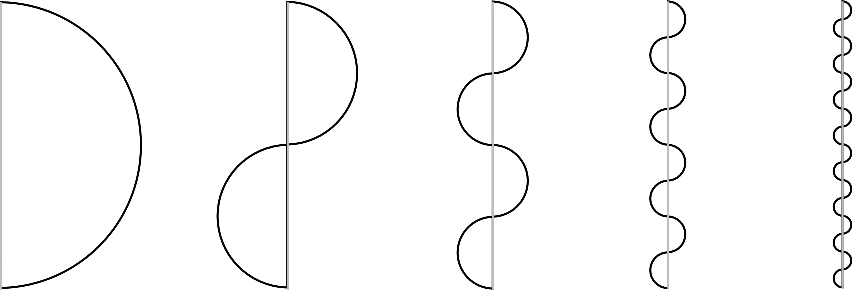
\includegraphics[width=.8\linewidth]{chapter2/figures/sequence.pdf}
\caption{Uniform convergence does not imply convergence in area. The
  sequence of curves converges uniformly to a straight line, but the
  length of the curves does not change.}
\label{fig:uniformconvergence}
\end{figure}


To the best of our knowledge, the only relevant results establish
convergence in area given convergence in vertex positions \emph{and}
convergence in normals, such as in Hildebrandt {\em et al.}
\cite{hildebrandt06}. However, the authors only establish
asymptotic convergence, with no order of accuracy associated with
it. The argument is more mathematically involved than space allows
here, so we refer the reader to that paper. Currently, this means that
the only information the observed order of accuracy provides to us is that
if we expect convergence in normals, we should also expect convergence
in area, and vice-versa.

% We assume once again that the isosurface $f(x,y,z)=\lambda$ can be written as
% the graph of a function $g(x(u,v),y(u,v))$ in $c_{ijk}$.

% %, one can compute the area of the isosurface in $c_{ijk}$ as follows:
% %\begin{equation}
% %\int\!\!\!\!\!\int_T \|\vec{n}\| dudv
% %\label{eq:area1}
% %\end{equation}
% %where $\vec{n}$ is the surface normal.
% The approximation error $E_a$ between the area of the exact surface 
% and the area of the triangle (as in Figure~\ref{fig:graphfunct})
% can be estimated using the traditional formula for the area of a parametric surface \cite{Courant},
% as follows: 
% \begin{equation}
% E_a = \left|\int\!\!\!\!\!\int_T \|\vec{n_{p_1p_2p_3}}\|- \|\vec{n}\| \;du\;dv\;\right|
% \label{eq:area1}
% \end{equation}
% \noindent where $T$ is the triangle defining the domain of $\vec{\Phi}$, $\vec{n_{p_1p_2p_3}}$ is 
% the normal of the triangle approximating the surface, and $\vec{n}$ is the normal 
% of the exact surface.

% Using (\ref{eq:normal_tri2}) and Taylor expansion for $\|\vec{n}\|$,
% together with the inequality $|a - b| \le |a| + |b|$, one can write:
% \begin{equation}
% E_a \le \left| \displaystyle{\int\!\!\!\!\!\int_T h^2(r\|\vec{n_0} + O(h)\| + \|\vec{n_0}\|+O(h)) \;du\;dv\;}\right| = O(h^2) \\
% \label{eq:area2}
% \end{equation}

% Therefore, from Equation (\ref{eq:area2}) one can see that the area of 
% the approximated surface has second order of accuracy.

\subsection{Convergence of Curvature}
\label{chap1:sec:curvconvergence}
The following formula gives an estimate of the curvature at a
vertex $p$:
\begin{equation}
K(p) = \frac{2\pi-\sum \theta_{i\,i+1}}{\frac{1}{3}A_{i\,i+1}}
\label{eq:curvat}
\end{equation}
\noindent where $\theta_{i\,i+1}$ and $A_{i\,i+1}$ are the angle 
$\angle p_ipp_{i+1}$ and area of the
triangle $p_ipp_{i+1}$ respectively (summation is over all triangles comprising 
the star of $p$)~\cite{meek2000}. 
Meek and Walton~\cite{meek2000} showed that the curvature computed via 
Equation~\ref{eq:curvat}
does not converge in general; that is, if the vertices of the star of $p$ 
are arbitrarily distributed
around $p$, one cannot expect curvature convergence. In fact, they
described a more general result stating that $O(h)$ accuracy can only be
obtained if the normals are known to have accuracy $O(h^2)$. Subsequently,
Xu~\cite{xu2006} presented a very particular distribution of vertices around $p$
under which the curvature estimated by Equation~\ref{eq:curvat} has accuracy $O(h^2)$. 

Curvature discretization schemes other than the one given in
Equation~\ref{eq:curvat} such as the quadratic-fit and spherical-image method
(see Meek and Walton~\cite{meek2000} for details) also demand
particular vertex distributions to ensure convergence. In our context
of keeping the analysis applicable for many isosurfacing algorithms,
this means we cannot use the lack of observed curvature convergence as an
indication of problematic behavior. Based on the results
mentioned above, one should actually expect curvature not to converge for most
isosurface extraction algorithms. More generally, this indicates a weakness of
MMS, namely that some features of interest (such as curvature)
will not have sufficient theoretical order of accuracy to be used in numerical
measurements. Notice, in addition, that if we had not written down the
theoretical model for curvature convergence, we might have expected
some sort of curvature approximation. Even a negative result such as
the one presented in this section can increase the confidence in the
results generated by an implementation.

% The convergence analysis of triangulated isosurfacing 
% can be accomplished by analyzing how quickly
% the triangular meshes converge to the original isosurface  
% when the background regular grid that supports the isosurface algorithm is 
% successively refined. Mathematically, 
% let $E_{S\tilde{S}_i}$ and $E_{S\tilde{S}_{i+1}}$ be the approximation errors of a given property
% $A:\mathbb{R}^3\rightarrow \mathbb{R}^d$ defined over $S$ and $\tilde{S}$
% in two consecutive grids with spacing $h_i$ and $h_{i+1}$ respectively, where 
% $h_{i+1} = \frac{h_i}{2}$. By conjecturing that the approximation error in two consecutive grids
% are related by:
% \begin{equation}
% E_{S\tilde{S}_{i+1}} = h^\alpha\, E_{S\tilde{S}_i}
% \label{eq:error-relation}
% \end{equation}
% \noindent where $h=h_1$ is the initial grid size, we define the convergence rate 
% (or error order) of the method as the exponent $\alpha$ in equation (\ref{eq:error-relation}).
% A typical approach to compute the convergence rate numerically is 
% to estimate $\alpha$ as the slope of the straight line
% that best fits the points $(\log h_i,\log E_{S\tilde{S}_i}),\; i=1\ldots s$, where $s$
% is the number of grids employed in the experiments.

